\documentclass{article}

\usepackage{graphicx}
\usepackage{tikz}
\usepackage{tikzsymbols}
\usetikzlibrary{calc,patterns,shapes.geometric}
\pagestyle{empty}
\usepackage[margin=0pt]{geometry}
\geometry{papersize={14in,12in}}

\def\centerarc[#1](#2)(#3:#4:#5){\draw[#1] ($(#2)+({#5*cos(#3)},{#5*sin(#3)})$) arc (#3:#4:#5);}

\begin{document}
	\begin{figure}
		\centering
		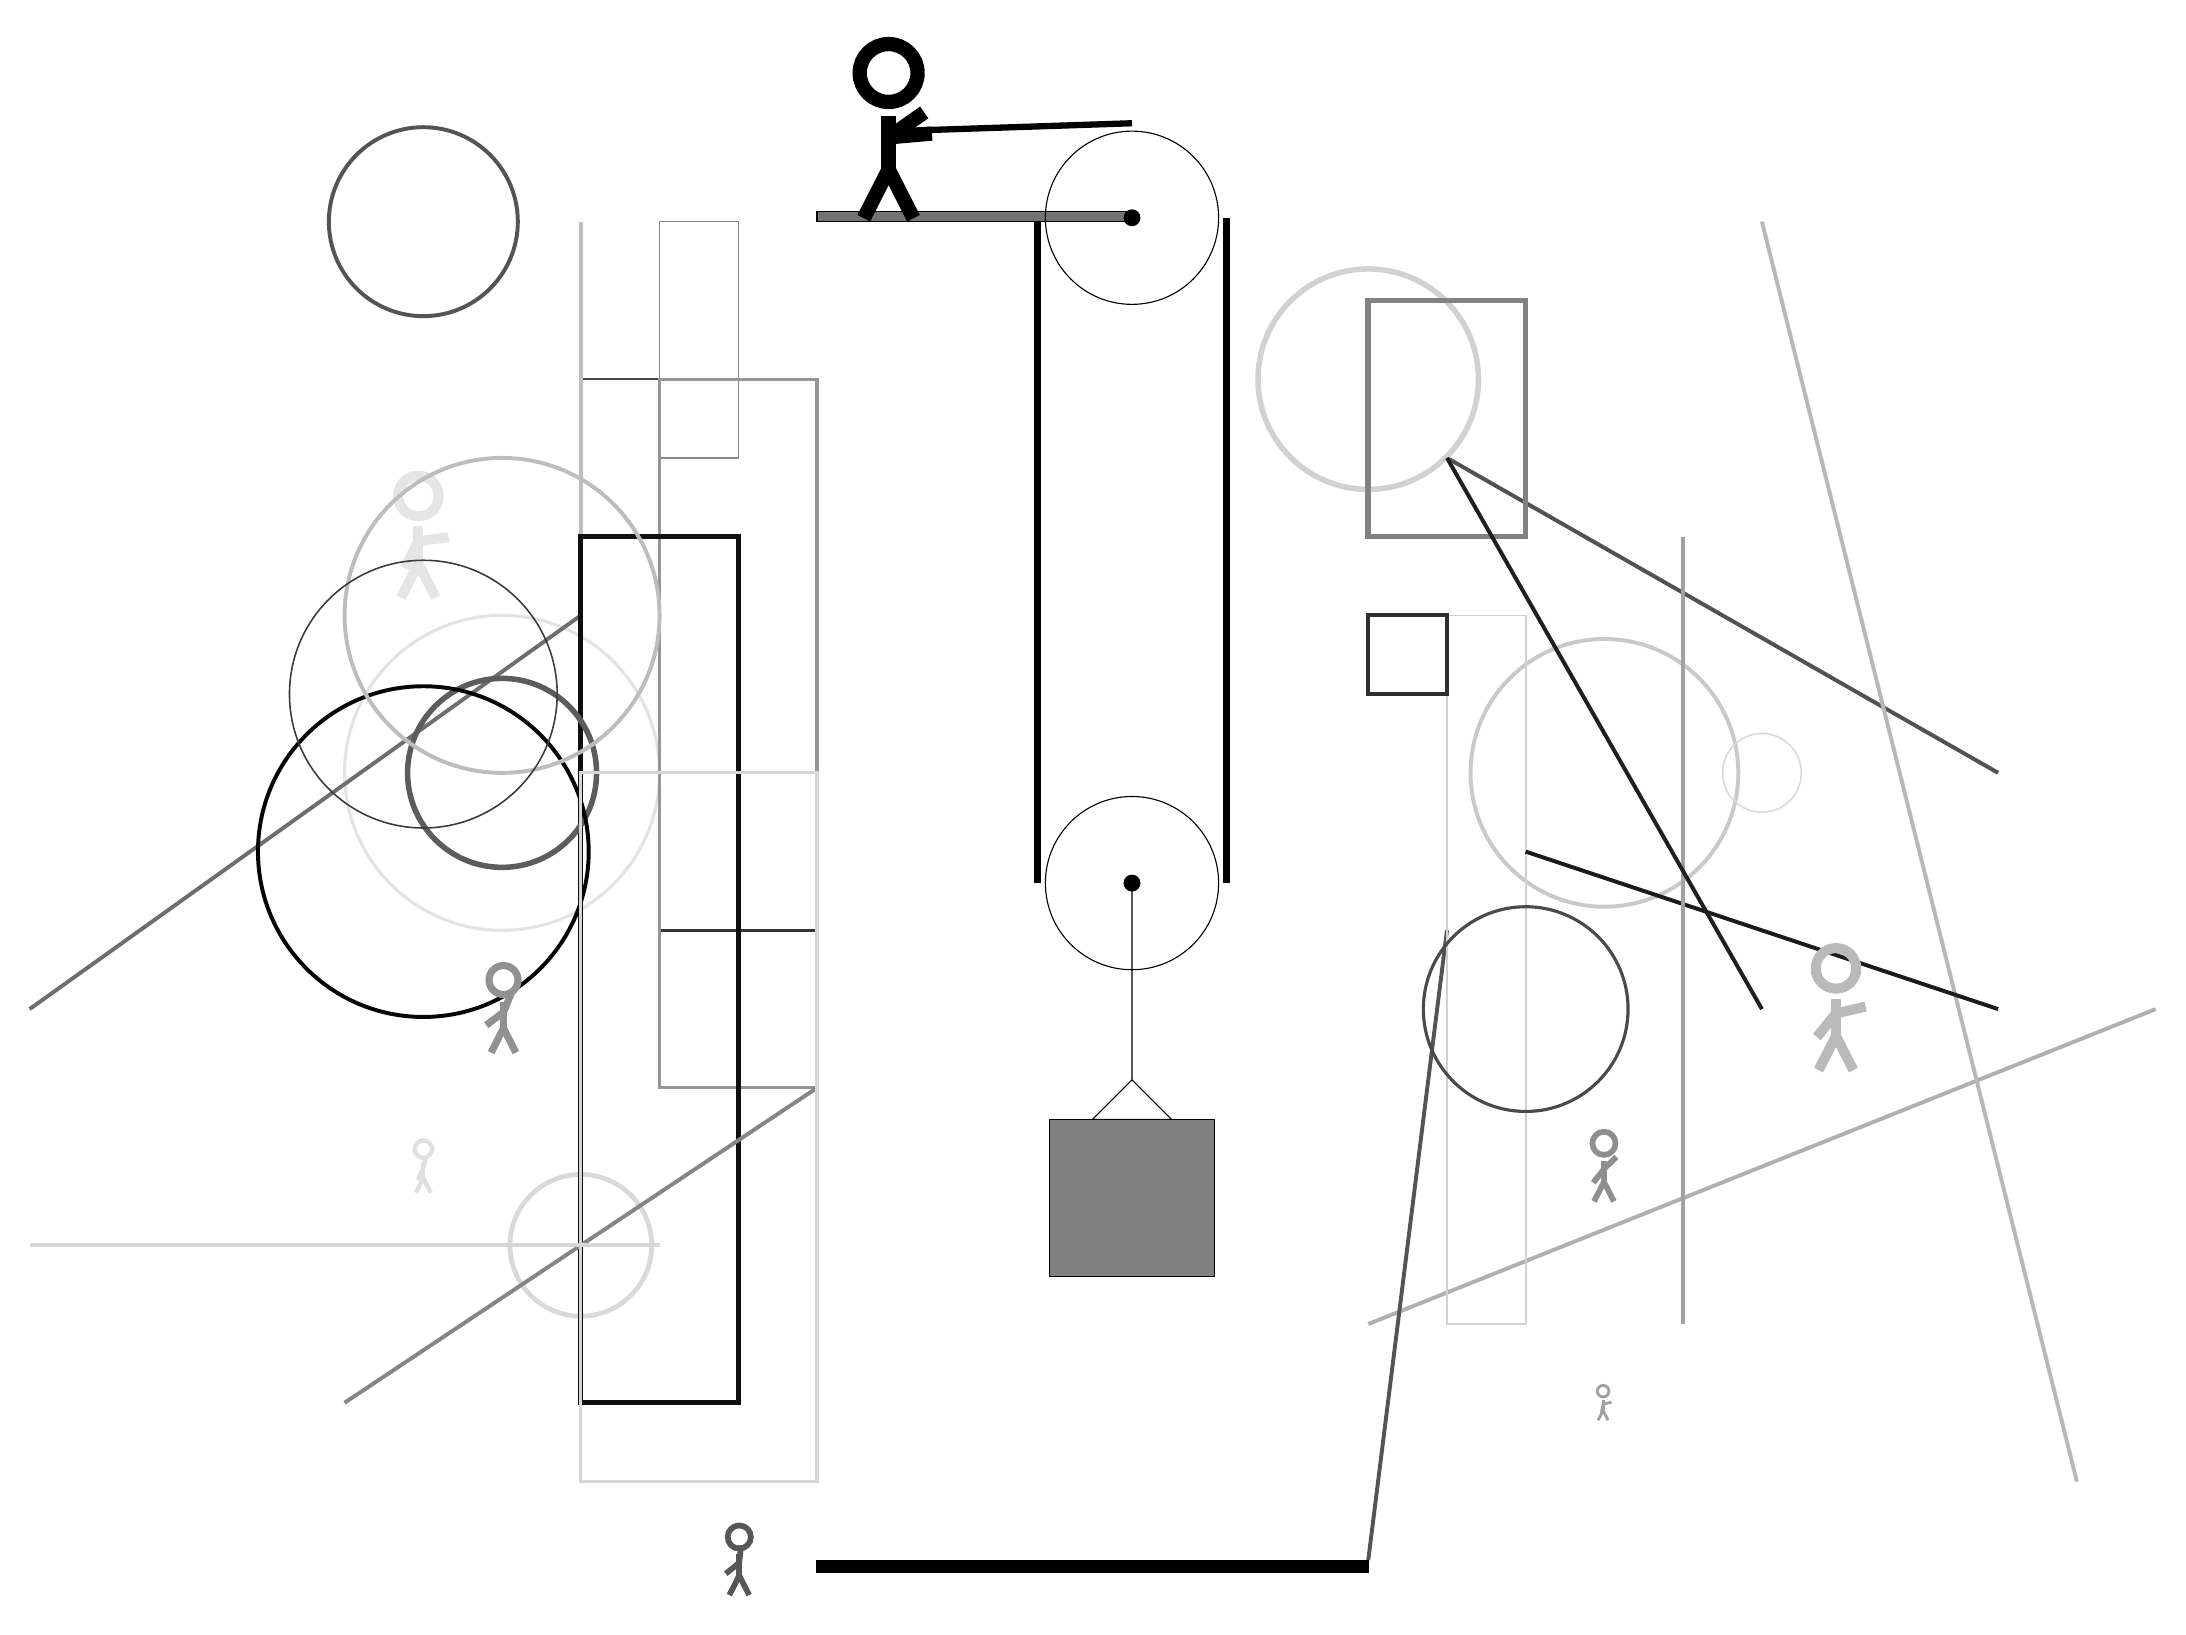
\begin{tikzpicture}
			%%%%% START %%%%%
			
			\draw[fill=black!55] (-2, 14) rectangle (2, 14.125);
			
			\draw[line width=0.4mm, color=black!79] (-4, 5) rectangle (-2, 12);
			
			\draw[line width=0.5mm, color=black!31](5, 0) -- (15, 4);
			\draw[line width=0.2mm, color=black!71] (-2, -2) rectangle (-5, 12);
			\draw [line width=0.4mm, color=black!11](-6, 7) circle (2.0);
			\draw[line width=0.5mm, color=black!57](-5, 9) -- (-12, 4);
			
			\node[line width=0.7mm, color=black!10] at (-7, 10) {\Strichmaxerl[7][63][7]};
			\draw[line width=0.2mm, color=black!47] (-4, 14) rectangle (-3, 11);
			\draw [line width=0.6mm, color=black!15](-5, 1) circle (0.9);
			\draw [line width=0.5mm, color=black!21](8, 7) circle (1.7);
			\draw[line width=0.5mm, color=black!68](6, 11) -- (13, 7);
			
			\node[line width=0.3mm, color=black!37] at (8, -1) {\Strichmaxerl[2][79][12]};
			
			\draw [line width=0.7mm, color=black!18](5, 12) circle (1.4);
			\node[line width=0.3mm, color=black!12] at (-7, 2) {\Strichmaxerl[3][64][78]};
			
			\draw[line width=0.5mm, color=black!25](-5, 7) -- (-5, 14);
			\draw[line width=0.4mm, color=black!41] (-4, 12) rectangle (-2, 3);
			\draw [line width=0.2mm, color=black!15](10, 7) circle (0.5);
			\draw[line width=0.5mm, color=black!67](5, -3) -- (6, 5);
			
			\node[line width=0.6mm, color=black!66] at (-3, -3) {\Strichmaxerl[4][39][84]};
			\draw[line width=0.6mm, color=black!94] (-3, -1) rectangle (-5, 10);
			\draw[line width=0.5mm, color=black!48](-2, 3) -- (-8, -1);
			\draw [line width=0.7mm, color=black!64](-6, 7) circle (1.2);
			
			\node[line width=0.2mm, color=black!44] at (8, 2) {\Strichmaxerl[4][52][44]};
			\draw[line width=0.2mm, color=black!18] (7, 9) rectangle (6, 0);
			\draw[line width=0.5mm, color=black!82] (6, 8) rectangle (5, 9);
			\draw[line width=0.5mm, color=black!28](10, 14) -- (14, -2);
			\draw[line width=0.5mm, color=black!89](7, 6) -- (13, 4);
			\draw[line width=0.5mm, color=black!16](-4, 1) -- (-12, 1);
			\draw [line width=0.5mm, color=black!98](-7, 6) circle (2.1);
			\draw[line width=0.5mm, color=black!37](9, 0) -- (9, 10);
			
			\draw [line width=0.5mm, color=black!26](-6, 9) circle (2.0);
			\node[line width=0.5mm, color=black!27] at (11, 4) {\Strichmaxerl[7][51][13]};
			\node[line width=0.6mm, color=black!43] at (-6, 4) {\Strichmaxerl[5][37][68]};
			\draw [line width=0.4mm, color=black!71](7, 4) circle (1.3);
			
			\draw[line width=0.4mm, color=black!16] (-2, 7) rectangle (-5, -2);
			
			\draw[line width=0.7mm, color=black!49] (7, 10) rectangle (5, 13);
			\draw [line width=0.5mm, color=black!67](-7, 14) circle (1.2);
			\draw [line width=0.2mm, color=black!77](-7, 8) circle (1.7);
			
			\draw[line width=0.5mm, color=black!88](6, 11) -- (10, 4);
			
			\draw (2, 5.6) circle (1.1);
			\draw[fill=black] (2, 5.6) circle (0.1);
			
			\draw (2, 14.05) circle (1.1);
			\draw[fill=black] (2, 14.05) circle (0.1);
			
			\draw (2, 5.6) -- (2, 3.1) -- (1.5, 2.6) -- (2.5, 2.6) -- (2, 3.1);
			\draw[fill=black!50] (0.95, 2.6) rectangle (3.05, 0.6);
			
			\draw[line width=0.8mm] (0.8, 14) -- (0.8, 5.6);
			\centerarc[line width=0.8mm](2, 5.6)(180:360:1.2000000000000002);
			\draw[line width=0.8mm](3.2, 5.6) -- (3.2, 14.05);
			\centerarc[line width=0.8mm](2, 14.05)(0:90:1.2000000000000002);
			\draw[line width=0.8mm](2, 15.25) -- (-1, 15.15);
			
			\node at (-1, 15.15) {\Strichmaxerl[10][-175][35]};
			
			\draw[fill=black] (-2, -3) rectangle (5, -3.15);
			
			%%%%% END %%%%%
		\end{tikzpicture}
	\end{figure}	
\end{document}